% Kommentare für den Editor (TexWorks/TexMakerX)
% !TeX encoding   = utf8
% !TeX spellcheck = de-DE

% --- LaTeX Vorlage ------------------------------------------------------
% speziell für einfache Dokumente wie Praktikumsprotokolle
%
% Autor: Matthias Pospiech (matthias@pospiech.eu)
% ------------------------------------------------------------------------

% Dokumentenklasse (Koma Script) -----------------------------------------
\documentclass[%
   %draft,     % Entwurfsstadium
   final,      % fertiges Dokument
   paper=a4, paper=portrait, pagesize=auto, % Papier Einstellungen
   fontsize=11pt, % Schriftgröße
   ngerman, % Sprache 
 ]{scrartcl} % Classes: scrartcl, scrreprt, scrbook

% ~~~~~~~~~~~~~~~~~~~~~~~~~~~~~~~~~~~~~~~~~~~~~~~~~~~~~~~~~~~~~~~~~~~~~~~~
% encoding
% ~~~~~~~~~~~~~~~~~~~~~~~~~~~~~~~~~~~~~~~~~~~~~~~~~~~~~~~~~~~~~~~~~~~~~~~~

% Encoding der Dateien (sonst funktionieren Umlaute nicht)
\usepackage[utf8]{inputenc}
\setlength\parindent{0pt} % Removes all indentation from paragraphs
\usepackage{listings}

\usepackage{tabularx}


\newcommand{\margin}{-0.5cm}
\newenvironment{changemargin}[2]{%
	\begin{list}{}{%
			\setlength{\topsep}{0pt}%
			\setlength{\leftmargin}{#1}%
			\setlength{\rightmargin}{#2}%
			\setlength{\listparindent}{\parindent}%
			\setlength{\itemindent}{\parindent}%
			\setlength{\parsep}{\parskip}%
		}%
		\item[]}{\end{list}}

% Encoding der Verzeichnisse (für Pfade mit Umlauten und Leerzeichne)
\usepackage[%
   extendedchars, encoding, multidot, space,
   filenameencoding=latin1, % Windows XP, Vista, 7
   % filenameencoding=utf8,   % Linux, OS X
]{grffile}

% ~~~~~~~~~~~~~~~~~~~~~~~~~~~~~~~~~~~~~~~~~~~~~~~~~~~~~~~~~~~~~~~~~~~~~~~~
% Pakete und Stile
% ~~~~~~~~~~~~~~~~~~~~~~~~~~~~~~~~~~~~~~~~~~~~~~~~~~~~~~~~~~~~~~~~~~~~~~~~
% Schriften
% ~~~~~~~~~~~~~~~~~~~~~~~~~~~~~~~~~~~~~~~~~~~~~~~~~~~~~~~~~~~~~~~~~~~~~~~~
% Fonts Fonts Fonts
% ~~~~~~~~~~~~~~~~~~~~~~~~~~~~~~~~~~~~~~~~~~~~~~~~~~~~~~~~~~~~~~~~~~~~~~~~

% immer laden:
\usepackage[T1]{fontenc} % T1 Schrift Encoding
\usepackage{textcomp}	 % Zusätzliche Symbole (Text Companion font extension)

% ~~~~~~~~~~~~~~~~~~~~~~~~~~~~~~~~~~~~~~~~~~~~~~~~~~~~~~~~~~~~~~~~~~~~~~~~
% Symbole
% ~~~~~~~~~~~~~~~~~~~~~~~~~~~~~~~~~~~~~~~~~~~~~~~~~~~~~~~~~~~~~~~~~~~~~~~~

\usepackage{amssymb}
\usepackage{mathcomp}


%% ==== Zusammengesetzte Schriften  (Sans + Serif) =======================

%% - Latin Modern
\usepackage{lmodern}
%% -------------------

%% - Bera Schriften
%\usepackage{bera}
%% -------------------

%% - Times, Helvetica, Courier (Word Standard...)
%\usepackage{mathptmx}
%\usepackage[scaled=.90]{helvet}
%\usepackage{courier}
%% -------------------

%% - Palantino , Helvetica, Courier
%\usepackage{mathpazo}
%\usepackage[scaled=.95]{helvet}
%\usepackage{courier}
%% -------------------

%% - Charter, Bera Sans
%\usepackage{charter}\linespread{1.05}
%\renewcommand{\sfdefault}{fvs}
%\usepackage[charter]{mathdesign}



%%%% =========== Typewriter =============

%\usepackage{courier}                   %% --- Courier
%\renewcommand{\ttdefault}{cmtl}        %% --- CmBright Typewriter Font
%\usepackage[%                          %% --- Luxi Mono (Typewriter)
%   scaled=0.9
%]{luximono}



% Pakete Laden
% ~~~~~~~~~~~~~~~~~~~~~~~~~~~~~~~~~~~~~~~~~~~~~~~~~~~~~~~~~~~~~~~~~~~~~~~~
% These packages must be loaded before all others
% (primarily because they are required by other packages)
% ~~~~~~~~~~~~~~~~~~~~~~~~~~~~~~~~~~~~~~~~~~~~~~~~~~~~~~~~~~~~~~~~~~~~~~~~
\usepackage{calc}
\usepackage{fixltx2e}	% Fix known LaTeX2e bugs

\usepackage[english]{babel} 			% Sprache
\usepackage[dvipsnames, table]{xcolor} 	% Farben

% ~~~~~~~~~~~~~~~~~~~~~~~~~~~~~~~~~~~~~~~~~~~~~~~~~~~~~~~~~~~~~~~~~~~~~~~~
% Hinzugefuegt bei mir (marvin)
% ~~~~~~~~~~~~~~~~~~~~~~~~~~~~~~~~~~~~~~~~~~~~~~~~~~~~~~~~~~~~~~~~~~~~~~~~


% ~~~~~~~~~~~~~~~~~~~~~~~~~~~~~~~~~~~~~~~~~~~~~~~~~~~~~~~~~~~~~~~~~~~~~~~~
% Bilder, Gleitumgebungen und Platzierung
% ~~~~~~~~~~~~~~~~~~~~~~~~~~~~~~~~~~~~~~~~~~~~~~~~~~~~~~~~~~~~~~~~~~~~~~~~

\usepackage[]{graphicx}					% Graphiken
\usepackage{epstopdf}		% konvertiert eps in pdf

% provides new floats and enables H float modifier option
\usepackage{float}
% Floats immer erst nach der Referenz setzen
\usepackage{flafter}
% Alel Floats werden vor der nächsten section ausgegeben
\usepackage[section]{placeins} 
%

% ~~~~~~~~~~~~~~~~~~~~~~~~~~~~~~~~~~~~~~~~~~~~~~~~~~~~~~~~~~~~~~~~~~~~~~~~
% Beschriftungen (captions)
% ~~~~~~~~~~~~~~~~~~~~~~~~~~~~~~~~~~~~~~~~~~~~~~~~~~~~~~~~~~~~~~~~~~~~~~~~

\usepackage{caption}
\usepackage{subcaption}

% ~~~~~~~~~~~~~~~~~~~~~~~~~~~~~~~~~~~~~~~~~~~~~~~~~~~~~~~~~~~~~~~~~~~~~~~~
% Math
% ~~~~~~~~~~~~~~~~~~~~~~~~~~~~~~~~~~~~~~~~~~~~~~~~~~~~~~~~~~~~~~~~~~~~~~~~

% Base Math Package
\usepackage[fleqn]{amsmath} 
% Warnt bei Benutzung von Befehlen die mit amsmath inkompatibel sind.
\usepackage[all, error]{onlyamsmath}

% ~~~~~~~~~~~~~~~~~~~~~~~~~~~~~~~~~~~~~~~~~~~~~~~~~~~~~~~~~~~~~~~~~~~~~~~~
% Science
% ~~~~~~~~~~~~~~~~~~~~~~~~~~~~~~~~~~~~~~~~~~~~~~~~~~~~~~~~~~~~~~~~~~~~~~~~

% Einheiten und Zahlenformatierung
\usepackage{siunitx}

% ~~~~~~~~~~~~~~~~~~~~~~~~~~~~~~~~~~~~~~~~~~~~~~~~~~~~~~~~~~~~~~~~~~~~~~~~
% Tables (Tabular)
% ~~~~~~~~~~~~~~~~~~~~~~~~~~~~~~~~~~~~~~~~~~~~~~~~~~~~~~~~~~~~~~~~~~~~~~~~

\usepackage{booktabs}
\usepackage{ltxtable} % Longtable + tabularx

% ~~~~~~~~~~~~~~~~~~~~~~~~~~~~~~~~~~~~~~~~~~~~~~~~~~~~~~~~~~~~~~~~~~~~~~~~
% text related packages
% ~~~~~~~~~~~~~~~~~~~~~~~~~~~~~~~~~~~~~~~~~~~~~~~~~~~~~~~~~~~~~~~~~~~~~~~~

\usepackage{url}            % Befehl \url{...}
\usepackage{enumitem}		% Kompakte Listen

% Neue Befehle: \Centering, \RaggedLeft, and \RaggedRight, ... 
\usepackage{ragged2e}


% ~~~~~~~~~~~~~~~~~~~~~~~~~~~~~~~~~~~~~~~~~~~~~~~~~~~~~~~~~~~~~~~~~~~~~~~~
% Citations
% ~~~~~~~~~~~~~~~~~~~~~~~~~~~~~~~~~~~~~~~~~~~~~~~~~~~~~~~~~~~~~~~~~~~~~~~~
%\usepackage[
%	style=alphabetic, % Loads the bibliography and the citation style 
%	natbib=true, % define natbib compatible cite commands
%]{biblatex}	
% Other options:
%	style=numeric, % 
%	style=numeric-comp,    % [1–3, 7, 8]
%	style=numeric-verb,    % [2]; [5]; [6]


% ~~~~~~~~~~~~~~~~~~~~~~~~~~~~~~~~~~~~~~~~~~~~~~~~~~~~~~~~~~~~~~~~~~~~~~~~
% layout packages
% ~~~~~~~~~~~~~~~~~~~~~~~~~~~~~~~~~~~~~~~~~~~~~~~~~~~~~~~~~~~~~~~~~~~~~~~~
%
% Befehle für 1,5 und 2 zeilig: 
% \singlespacing, \onehalfspacing und \doublespacing
\usepackage{setspace}

% ~~~~~~~~~~~~~~~~~~~~~~~~~~~~~~~~~~~~~~~~~~~~~~~~~~~~~~~~~~~~~~~~~~~~~~~~
% Kopf und Fusszeile
% ~~~~~~~~~~~~~~~~~~~~~~~~~~~~~~~~~~~~~~~~~~~~~~~~~~~~~~~~~~~~~~~~~~~~~~~~

% Kopf und Fusszeile mit scrpage2 einstellen
\usepackage[automark, komastyle, nouppercase]{scrpage2}

% ~~~~~~~~~~~~~~~~~~~~~~~~~~~~~~~~~~~~~~~~~~~~~~~~~~~~~~~~~~~~~~~~~~~~~~~~
% pdf packages
% ~~~~~~~~~~~~~~~~~~~~~~~~~~~~~~~~~~~~~~~~~~~~~~~~~~~~~~~~~~~~~~~~~~~~~~~~

% Include pages from external PDF documents in LaTeX documents
\usepackage{pdfpages} 

% Optischer Randausgleich mit pdfTeX
\usepackage{microtype}

% Links
\usepackage[hidelinks]{hyperref}

% Einstellungen und Layoutstile 
% ~~~~~~~~~~~~~~~~~~~~~~~~~~~~~~~~~~~~~~~~~~~~~~~~~~~~~~~~~~~~~~~~~~~~~~~~
% Colors
% ~~~~~~~~~~~~~~~~~~~~~~~~~~~~~~~~~~~~~~~~~~~~~~~~~~~~~~~~~~~~~~~~~~~~~~~~
\definecolor{sectioncolor}{RGB}{0, 0, 0}     % black

% ~~~~~~~~~~~~~~~~~~~~~~~~~~~~~~~~~~~~~~~~~~~~~~~~~~~~~~~~~~~~~~~~~~~~~~~~
% text related 
% ~~~~~~~~~~~~~~~~~~~~~~~~~~~~~~~~~~~~~~~~~~~~~~~~~~~~~~~~~~~~~~~~~~~~~~~~

%% style of URL
\urlstyle{tt}


% Keine hochgestellten Ziffern in der Fussnote (KOMA-Script-spezifisch):
\deffootnote{1.5em}{1em}{\makebox[1.5em][l]{\thefootnotemark}}

% Limit space of footnotes to 10 lines
\setlength{\dimen\footins}{10\baselineskip}

% prevent continuation of footnotes 
% at facing page
\interfootnotelinepenalty=10000 

% ~~~~~~~~~~~~~~~~~~~~~~~~~~~~~~~~~~~~~~~~~~~~~~~~~~~~~~~~~~~~~~~~~~~~~~~~
% Science
% ~~~~~~~~~~~~~~~~~~~~~~~~~~~~~~~~~~~~~~~~~~~~~~~~~~~~~~~~~~~~~~~~~~~~~~~~

\sisetup{%
	mode = math, detect-family, detect-weight,	
	exponent-product = \cdot,
	number-unit-separator=\text{\,},
	output-decimal-marker={,},
}

% ~~~~~~~~~~~~~~~~~~~~~~~~~~~~~~~~~~~~~~~~~~~~~~~~~~~~~~~~~~~~~~~~~~~~~~~~
% Citations / Style of Bibliography
% ~~~~~~~~~~~~~~~~~~~~~~~~~~~~~~~~~~~~~~~~~~~~~~~~~~~~~~~~~~~~~~~~~~~~~~~~

% Kommentar entfernene wenn biblatex geladen wird
% \IfPackageLoaded{biblatex}{%
	\ExecuteBibliographyOptions{%
%--- Backend --- --- ---
	backend=bibtex,  % (bibtex, bibtex8, biber)
	bibwarn=true, %
	bibencoding=ascii, % (ascii, inputenc, <encoding>)
%--- Sorting --- --- ---
	sorting=nty, % Sort by name, title, year.
	% other options: 
	% nty        Sort by name, title, year.
	% nyt        Sort by name, year, title.
	% nyvt       Sort by name, year, volume, title.
	% anyt       Sort by alphabetic label, name, year, title.
	% anyvt      Sort by alphabetic label, name, year, volume, title.
	% ynt        Sort by year, name, title.
	% ydnt       Sort by year (descending), name, title.
	% none       Do not sort at all. All entries are processed in citation order.
	% debug      Sort by entry key. This is intended for debugging only.
	%
	sortcase=true,
	sortlos=los, % (bib, los) The sorting order of the list of shorthands
	sortcites=false, % do/do not sort citations according to bib	
%--- Dates --- --- ---
	date=comp,  % (short, long, terse, comp, iso8601)
%	origdate=
%	eventdate=
%	urldate=
%	alldates=
	datezeros=true, %
	dateabbrev=true, %
%--- General Options --- --- ---
	maxnames=1,
	minnames=1,
%	maxbibnames=99,
%	maxcitenames=1,
%	autocite= % (plain, inline, footnote, superscript) 
	autopunct=true,
	language=auto,
	babel=none, % (none, hyphen, other, other*)
	block=none, % (none, space, par, nbpar, ragged)
	notetype=foot+end, % (foot+end, footonly, endonly)
	hyperref=true, % (true, false, auto)
	backref=true,
	backrefstyle=three, % (none, three, two, two+, three+, all+)
	backrefsetstyle=setonly, %
	indexing=false, % 
	% options:
	% true       Enable indexing globally.
	% false      Disable indexing globally.
	% cite       Enable indexing in citations only.
	% bib        Enable indexing in the bibliography only.
	refsection=none, % (part, chapter, section, subsection)
	refsegment=none, % (none, part, chapter, section, subsection)
	abbreviate=true, % (true, false)
	defernumbers=false, % 
	punctfont=false, % 
	arxiv=abs, % (ps, pdf, format)	
%--- Style Options --- --- ---	
% The following options are provided by the standard styles
	isbn=false,%
	url=false,%
	doi=false,%
	eprint=false,%	
	}%	
	
	% change alpha label to be without +	
	\renewcommand*{\labelalphaothers}{}
	
	% change 'In: <magazine>" to "<magazine>"
	\renewcommand*{\intitlepunct}{}
	\DefineBibliographyStrings{german}{in={}}
	
	% make names capitalized \textsc{}
	\renewcommand{\mkbibnamefirst}{\textsc}
	\renewcommand{\mkbibnamelast}{\textsc}
	
	% make volume and number look like 
	% 'Bd. 33(14): '
	\renewbibmacro*{volume+number+eid}{%
	  \setunit{\addcomma\space}%
	  \bibstring{volume}% 
	  \setunit{\addspace}%
	  \printfield{volume}%
	  \iffieldundef{number}{}{% 
	    \printtext[parens]{%
	      \printfield{number}%
	    }%
	  }%
	  \setunit{\addcomma\space}%
	  \printfield{eid}
	  %\setunit{\addcolon\space}%
	  }	

	% <authors>: <title>
	\renewcommand*{\labelnamepunct}{\addcolon\space}
	% make ': ' before pages
	\renewcommand*{\bibpagespunct}{\addcolon\space}
	% names delimiter ';' instead of ','
	%\renewcommand*{\multinamedelim}{\addsemicolon\space}

	% move date before issue
	\renewbibmacro*{journal+issuetitle}{%
	  \usebibmacro{journal}%
	  \setunit*{\addspace}%
	  \iffieldundef{series}
	    {}
	    {\newunit
	     \printfield{series}%
	     \setunit{\addspace}}%
	  %
	  \usebibmacro{issue+date}%
	  \setunit{\addcolon\space}%
	  \usebibmacro{issue}%
	  \setunit{\addspace}%
	  \usebibmacro{volume+number+eid}%
	  \newunit}

	% print all names, even if maxnames = 1
	\DeclareCiteCommand{\citeauthors}
	  {
	   \defcounter{maxnames}{1000}
	   \boolfalse{citetracker}%
	   \boolfalse{pagetracker}%
	   \usebibmacro{prenote}}
	  {\ifciteindex
	     {\indexnames{labelname}}
	     {}%
	   \printnames{labelname}}
	  {\multicitedelim}
	  {\usebibmacro{postnote}}

}%

% ~~~~~~~~~~~~~~~~~~~~~~~~~~~~~~~~~~~~~~~~~~~~~~~~~~~~~~~~~~~~~~~~~~~~~~~~
% figures, placement, floats and captions
% ~~~~~~~~~~~~~~~~~~~~~~~~~~~~~~~~~~~~~~~~~~~~~~~~~~~~~~~~~~~~~~~~~~~~~~~~

% Make float placement easier
\renewcommand{\floatpagefraction}{.75} % vorher: .5
\renewcommand{\textfraction}{.1}       % vorher: .2
\renewcommand{\topfraction}{.8}        % vorher: .7
\renewcommand{\bottomfraction}{.5}     % vorher: .3
\setcounter{topnumber}{3}        % vorher: 2
\setcounter{bottomnumber}{2}     % vorher: 1
\setcounter{totalnumber}{5}      % vorher: 3

%% ~~~ Captions ~~~~~~~~~~~~~~~~~~~~~~~~~~~~~~~~~~~~~~~~~~~~~~~~~~~~~~~~~~
% Style of captions
\DeclareCaptionStyle{captionStyleTemplateDefault}
[ % single line captions
   justification = centering
]
{ % multiline captions
% -- Formatting
   format      = plain,  % plain, hang
   indention   = 0em,    % indention of text 
   labelformat = default,% default, empty, simple, brace, parens
   labelsep    = colon,  % none, colon, period, space, quad, newline, endash
   textformat  = simple, % simple, period
% -- Justification
   justification = justified, %RaggedRight, justified, centering
   singlelinecheck = true, % false (true=ignore justification setting in single line)
% -- Fonts
   labelfont   = {small,bf},
   textfont    = {small,rm},
% valid values:
% scriptsize, footnotesize, small, normalsize, large, Large
% normalfont, ip, it, sl, sc, md, bf, rm, sf, tt
% singlespacing, onehalfspacing, doublespacing
% normalcolor, color=<...>
%
% -- Margins and further paragraph options
   margin = 10pt, %.1\textwidth,
   % width=.8\linewidth,
% -- Skips
   skip     = 10pt, % vertical space between the caption and the figure
   position = auto, % top, auto, bottom
% -- Lists
   % list=no, % suppress any entry to list of figure 
   listformat = subsimple, % empty, simple, parens, subsimple, subparens
% -- Names & Numbering
   % figurename = Abb. %
   % tablename  = Tab. %
   % listfigurename=
   % listtablename=
   % figurewithin=chapter
   % tablewithin=chapter
%-- hyperref related options
	hypcap=true, % (true, false) 
	% true=all hyperlink anchors are placed at the 
	% beginning of the (floating) environment
	%
	hypcapspace=0.5\baselineskip
}

% apply caption style
\captionsetup{
	style = captionStyleTemplateDefault % base
}

% Predefinded skip setup for different floats
\captionsetup[table]{position=top}
\captionsetup[figure]{position=bottom}


% options for subcaptions
\captionsetup[sub]{ %
	style = captionStyleTemplateDefault, % base
	skip=6pt,
	margin=5pt,
	labelformat = parens,% default, empty, simple, brace
	labelsep    = space,
	list=false,
	hypcap=false
}

% ~~~~~~~~~~~~~~~~~~~~~~~~~~~~~~~~~~~~~~~~~~~~~~~~~~~~~~~~~~~~~~~~~~~~~~~~
% layout 
% ~~~~~~~~~~~~~~~~~~~~~~~~~~~~~~~~~~~~~~~~~~~~~~~~~~~~~~~~~~~~~~~~~~~~~~~~


%% Paragraph Separation =================================
\KOMAoptions{%
   parskip=absolute, % do not change indentation according to fontsize
   parskip=false     % indentation of 1em
   % parskip=half    % parksip of 1/2 line 
}%

%% line spacing =========================================
%\onehalfspacing	% 1,5-facher Abstand
%\doublespacing		% 2-facher Abstand

%% page layout ==========================================

\raggedbottom     % Variable Seitenhoehen zulassen

% Koma Script text area layout
\KOMAoptions{%
   DIV=14,% (Size of Text Body, higher values = greater textbody)
   BCOR=5mm% (Bindekorrektur)
}%

%%% === Page Layout  Options ===
\KOMAoptions{% (most options are for package typearea)
   % twoside=true, % two side layout (alternating margins, standard in books)
   %oneside=true, % single side layout 
   %
   headlines=2.1,%
}%

%\KOMAoptions{%
%      headings=noappendixprefix % chapter in appendix as in body text
%      ,headings=nochapterprefix  % no prefix at chapters
%      % ,headings=appendixprefix   % inverse of 'noappendixprefix'
%      % ,headings=chapterprefix    % inverse of 'nochapterprefix'
%      % ,headings=openany   % Chapters start at any side
%      % ,headings=openleft  % Chapters start at left side
%      ,headings=openright % Chapters start at right side      
%}%


% reloading of typearea, necessary if setting of spacing changed
\typearea[current]{last}

% ~~~~~~~~~~~~~~~~~~~~~~~~~~~~~~~~~~~~~~~~~~~~~~~~~~~~~~~~~~~~~~~~~~~~~~~~
% Titlepage
% ~~~~~~~~~~~~~~~~~~~~~~~~~~~~~~~~~~~~~~~~~~~~~~~~~~~~~~~~~~~~~~~~~~~~~~~~
\KOMAoptions{%
   % titlepage=true %
   titlepage=false %
}%

% ~~~~~~~~~~~~~~~~~~~~~~~~~~~~~~~~~~~~~~~~~~~~~~~~~~~~~~~~~~~~~~~~~~~~~~~~
% head and foot lines
% ~~~~~~~~~~~~~~~~~~~~~~~~~~~~~~~~~~~~~~~~~~~~~~~~~~~~~~~~~~~~~~~~~~~~~~~~

% \pagestyle{scrheadings} % Seite mit Headern
\pagestyle{scrplain} % Seiten ohne Header

% loescht voreingestellte Stile
\clearscrheadings
\clearscrplain
%
% Was steht wo...
% Bei headings:
%   % Oben aussen: Kapitel und Section
%   % Unten aussen: Seitenzahl
%   \ohead{\pagemark}
%   \ihead{\headmark}
%   \ofoot[\pagemark]{} % Außen unten: Seitenzahlen bei plain
% Bei Plain:
\cfoot[\pagemark]{\pagemark} % Mitte unten: Seitenzahlen bei plain


% Angezeigte Abschnitte im Header
% \automark[section]{chapter} %[rechts]{links}
\automark[subsection]{section} %[rechts]{links}

% ~~~~~~~~~~~~~~~~~~~~~~~~~~~~~~~~~~~~~~~~~~~~~~~~~~~~~~~~~~~~~~~~~~~~~~~~
% headings / page opening
% ~~~~~~~~~~~~~~~~~~~~~~~~~~~~~~~~~~~~~~~~~~~~~~~~~~~~~~~~~~~~~~~~~~~~~~~~
\setcounter{secnumdepth}{2}

\KOMAoptions{%
%%%% headings
   % headings=small  % Small Font Size, thin spacing above and below
   % headings=normal % Medium Font Size, medium spacing above and below
   headings=big % Big Font Size, large spacing above and below
}%

% Titelzeile linksbuendig, haengend
\renewcommand*{\raggedsection}{\raggedright} 
\setlength\parindent{0pt}
% ~~~~~~~~~~~~~~~~~~~~~~~~~~~~~~~~~~~~~~~~~~~~~~~~~~~~~~~~~~~~~~~~~~~~~~~~
% fonts of headings
% ~~~~~~~~~~~~~~~~~~~~~~~~~~~~~~~~~~~~~~~~~~~~~~~~~~~~~~~~~~~~~~~~~~~~~~~~
\setkomafont{sectioning}{\normalfont\sffamily} % \rmfamily
\setkomafont{descriptionlabel}{\itshape}
\setkomafont{pageheadfoot}{\normalfont\normalcolor\small\sffamily}
\setkomafont{pagenumber}{\normalfont\sffamily}

%%% --- Titlepage ---
%\setkomafont{subject}{}
%\setkomafont{subtitle}{}
%\setkomafont{title}{}

% ~~~~~~~~~~~~~~~~~~~~~~~~~~~~~~~~~~~~~~~~~~~~~~~~~~~~~~~~~~~~~~~~~~~~~~~~
% settings and layout of TOC, LOF, 
% ~~~~~~~~~~~~~~~~~~~~~~~~~~~~~~~~~~~~~~~~~~~~~~~~~~~~~~~~~~~~~~~~~~~~~~~~
\setcounter{tocdepth}{3} % Depth of TOC Display

% ~~~~~~~~~~~~~~~~~~~~~~~~~~~~~~~~~~~~~~~~~~~~~~~~~~~~~~~~~~~~~~~~~~~~~~~~
% Tabellen
% ~~~~~~~~~~~~~~~~~~~~~~~~~~~~~~~~~~~~~~~~~~~~~~~~~~~~~~~~~~~~~~~~~~~~~~~~

%%% -| Neue Spaltendefinitionen 'columntypes' |--
%
% Belegte Spaltentypen:
% l - links
% c - zentriert
% r - rechts
% p,m,b  - oben, mittig, unten
% X - tabularx Auto-Spalte

% um Tabellenspalten mit Flattersatz zu setzen, muss \\ vor
% (z.B.) \raggedright geschuetzt werden:
\newcommand{\PreserveBackslash}[1]{\let\temp=\\#1\let\\=\temp}

% Spalten mit Flattersatz und definierte Breite:
% m{} -> mittig
% p{} -> oben
% b{} -> unten
%
% Linksbuendig:
\newcolumntype{v}[1]{>{\PreserveBackslash\RaggedRight\hspace{0pt}}p{#1}}
\newcolumntype{M}[1]{>{\PreserveBackslash\RaggedRight\hspace{0pt}}m{#1}}
% % Rechtsbuendig :
% \newcolumntype{R}[1]{>{\PreserveBackslash\RaggedLeft\hspace{0pt}}m{#1}}
% \newcolumntype{S}[1]{>{\PreserveBackslash\RaggedLeft\hspace{0pt}}p{#1}}
% % Zentriert :
% \newcolumntype{Z}[1]{>{\PreserveBackslash\Centering\hspace{0pt}}m{#1}}
% \newcolumntype{A}[1]{>{\PreserveBackslash\Centering\hspace{0pt}}p{#1}}

\newcolumntype{Y}{>{\PreserveBackslash\RaggedLeft\hspace{0pt}}X}

%-- Einstellungen für Tabellen ----------
\providecommand\tablestyle{%
  \renewcommand{\arraystretch}{1.4} % Groessere Abstaende zwischen Zeilen
  \normalfont\normalsize            %
  \sffamily\small           % Serifenlose und kleine Schrift
  \centering%                       % Tabelle zentrieren
}

%--Einstellungen für Tabellen ----------

\colorlet{tablesubheadcolor}{gray!40}
\colorlet{tableheadcolor}{gray!25}
\colorlet{tableblackheadcolor}{black!60}
\colorlet{tablerowcolor}{gray!15.0}


% ~~~~~~~~~~~~~~~~~~~~~~~~~~~~~~~~~~~~~~~~~~~~~~~~~~~~~~~~~~~~~~~~~~~~~~~~
% pdf packages
% ~~~~~~~~~~~~~~~~~~~~~~~~~~~~~~~~~~~~~~~~~~~~~~~~~~~~~~~~~~~~~~~~~~~~~~~~

% ~~~~~~~~~~~~~~~~~~~~~~~~~~~~~~~~~~~~~~~~~~~~~~~~~~~~~~~~~~~~~~~~~~~~~~~~
% fix remaining problems
% ~~~~~~~~~~~~~~~~~~~~~~~~~~~~~~~~~~~~~~~~~~~~~~~~~~~~~~~~~~~~~~~~~~~~~~~~




% ~~~~~~~~~~~~~~~~~~~~~~~~~~~~~~~~~~~~~~~~~~~~~~~~~~~~~~~~~~~~~~~~~~~~~~~~
% Eigene Befehle
% ~~~~~~~~~~~~~~~~~~~~~~~~~~~~~~~~~~~~~~~~~~~~~~~~~~~~~~~~~~~~~~~~~~~~~~~~
% -- new commands --
\providecommand{\abs}[1]{\lvert#1\rvert}
\providecommand{\Abs}[1]{\left\lvert#1\right\rvert}
\providecommand{\norm}[1]{\left\Vert#1\right\Vert}
\providecommand{\Trace}[1]{\ensuremath{\Tr\{\,#1\,\}}} % Trace /Spur
%

\renewcommand{\d}{\partial\mspace{2mu}} % partial diff
\newcommand{\td}{\,\mathrm{d}}	% total diff

\newcommand{\Ham}{\mathcal{H}}    % Hamilton
\newcommand{\Prob}{\mathscr{P}}    % Hamilton
\newcommand{\unity}{\mathds{1}}   % Real

\renewcommand{\i}{\mathrm{i}}   % imagin�re Einheit



% -- New Operators --
\DeclareMathOperator{\rot}{rot}
\DeclareMathOperator{\grad}{grad}
\DeclareMathOperator{\Tr}{Tr}
\DeclareMathOperator{\const}{const}
\DeclareMathOperator{\e}{e} 			% exponatial Function




\usepackage{listings}
\usepackage{color}

% color definitions and code style
\definecolor{codeblue}{RGB}{58,33,158}
\definecolor{codegreen}{rgb}{0,0.47,0}
\definecolor{codegray}{rgb}{0.5,0.5,0.5}
\definecolor{codepurple}{rgb}{0.55,0,0.53}
\definecolor{backcolour}{rgb}{0.97,0.97,0.97}

\lstdefinestyle{vhdlstyle}{
	basicstyle=\small,
	backgroundcolor=\color{backcolour},
	commentstyle=\color{deepred},
	keywordstyle=\color{codepurple},
	numberstyle=\tiny\color{codegray},
	stringstyle=\color{codegreen},
	breakatwhitespace=false,         
	breaklines=true,                 
	captionpos=b,                    
	keepspaces=true,                
	showspaces=false,                
	showstringspaces=false,
	showtabs=false,                  
	tabsize=2,
	emphstyle=\color{codeblue},
	frame=single,
	captionpos=t,
	% language specific
	language=vhdl,
	otherkeywords={},
	emph={}
}

\lstdefinestyle{cppstyle}{
	basicstyle=\small,
	backgroundcolor=\color{backcolour},
	commentstyle=\color{deepred},
	keywordstyle=\color{codepurple},
	numberstyle=\tiny\color{codegray},
	stringstyle=\color{codegreen},
	breakatwhitespace=false,         
	breaklines=true,                 
	captionpos=b,                    
	keepspaces=true,                
	showspaces=false,                
	showstringspaces=false,
	showtabs=false,                  
	tabsize=2,
	emphstyle=\color{codeblue},
	frame=single,
	captionpos=t,
	% language specific
	language=c++,
	otherkeywords={emit,override,TEST_CASE,SECTION,REQUIRE,Q_OBJECT,;,\{,\},+,-,*,/},
	emph={MeasurementDevice,ScpiDevice,quint64,Serial,QThread,QWidget,QMap,quint32,QPointer,DeviceParameterConstraint, MeasurementValue,DeviceManager,QString,QPointer,QStringList,std, Dummy, Keithley_2000, Keithley_2410, SourceTronic_ST2819A, Tektronix_DMM4020, Voltcraft_PSP1803, RIGOL_DSA1030A, HP_34401A, Hameg_HM8143, GW_INSTEK_GPD4303S}
}

\lstdefinestyle{pythonstyle}{
	basicstyle=\small,
	backgroundcolor=\color{backcolour},
	commentstyle=\color{deepred},
	keywordstyle=\color{codepurple},
	numberstyle=\tiny\color{codegray},
	stringstyle=\color{codegreen},
	breakatwhitespace=false,         
	breaklines=true,                 
	captionpos=b,                    
	keepspaces=true,                
	showspaces=false,                
	showstringspaces=false,
	showtabs=false,                  
	tabsize=2,
	emphstyle=\color{codeblue},
	frame=single,
	captionpos=t,
	% language specific
	language=Python,
	otherkeywords={},
	emph={}
}

% VHDL environment
\lstnewenvironment{vhdl} {
	\lstset{style=vhdlstyle}
}{}

% Python environment
\lstnewenvironment{python} {
	\lstset{style=pythonstyle}
}{}
%c++ environment
\lstnewenvironment{cpp} {
	\lstset{style=cppstyle}
}{}

% ~~~~~~~~~~~~~~~~~~~~~~~~~~~~~~~~~~~~~~~~~~~~~~~~~~~~~~~~~~~~~~~~~~~~~~~~
% Eigene Befehle
% ~~~~~~~~~~~~~~~~~~~~~~~~~~~~~~~~~~~~~~~~~~~~~~~~~~~~~~~~~~~~~~~~~~~~~~~~
% Silbentrennung hinzufügen als 
% Sil-ben-tren-nung 
\hyphenation{}

\listfiles % schreibt alle verwendeten Dateien in die log Datei


% custom fonts and math extensions
\usepackage{fontspec}
\usepackage{unicode-math} 
\usepackage{amsmath}                % Für fancy Formel-Umgebungen.
\usepackage{amssymb}                % Für fancy Mathe-Zeichen.
\usepackage{amsfonts}               % Für fancy Mathe-Schrift im math mode (Cambria Math)
\usepackage{siunitx}

\newfontfamily{\amethysta}{Amethysta-Regular}
[Path = fonts/amethysta/, Extension = .ttf]
\DeclareTextFontCommand{\textdedication}{\amethysta}

%\newfontfamily{\computermodern}{cmunrm}
%[Path = fonts/computer-modern/, Extension = .ttf]
%\DeclareTextFontCommand{\textdedication}{\computermodern}

\usepackage{pifont}
\newcommand{\cmark}{\ding{51}}%
\newcommand{\xmark}{\ding{55}}%

\newfontfamily{\polyglott}{polyglott}
[Path = fonts/polyglott/, Extension = .ttf]
\DeclareTextFontCommand{\textdedication}{\polyglott}

\setmainfont[Path = fonts/amethysta/, Extension = .ttf]{Amethysta-Regular}
%\setmainfont[Path = fonts/cormorant/, Extension = .ttf]{Cormorant-Regular}
\setmathfont{Cambria Math}

% select toc font
\usepackage{tocloft,lipsum,pgffor,sectsty}

\setcounter{tocdepth}{2}% Include up to \subsection in ToC

% Font changes to ToC content of sectional units
\renewcommand{\cftpartfont}{\polyglott\bfseries}% \part font in ToC
\renewcommand{\cftsecfont}{\normalfont\sffamily\large\bfseries}           % \section font in ToC
\renewcommand{\cftsubsecfont}{\normalfont\sffamily\large}        % \subsection font in ToC
%\renewcommand{\cftsubsubsecfont}{\polyglott\small}       % \subsubsection font in ToC

% Font changes to document content of sectional units
\renewcommand{\partfont}{\normalfont\sffamily\Huge\bfseries}
\renewcommand{\sectionfont}{\normalfont\sffamily\Huge\bfseries}

\usepackage{titlesec}

\titleformat*{\section}{\sffamily\LARGE\bfseries}
\titleformat*{\subsection}{\sffamily\Large\bfseries}
\titleformat*{\subsubsection}{\sffamily\large\bfseries}
\titleformat*{\paragraph}{\sffamily\large\bfseries}
\titleformat*{\subparagraph}{\sffamily\large\bfseries}

%% Dokument Beginn %%%%%%%%%%%%%%%%%%%%%%%%%%%%%%%%%%%%%%%%%%%%%%%%%%%%%%%%
\begin{document}	

\graphicspath{{content/figures/}} % Location of the graphics files {{}} because of windows

% Automatische Titelseite

\title{General Purpose Control GUI for tabletop lab devices and more}
\author{Marvin Peter}
\date{\today}
\maketitle
\begin{figure}[h]
	\centering
	\includegraphics[scale=0.5]{content/figures/jlu-logo.ps}
\end{figure}
\thispagestyle{empty}
\newpage
{\tableofcontents}
\thispagestyle{empty}
\newcommand{\env}[1]{\texttt{#1}}
\newcommand{\command}[1]{\texttt{#1}}
\newcommand{\package}[1]{\texttt{\itshape#1}}
\newcommand{\engl}[1]{(engl: \textit{#1})\xspace}
\newpage

\setcounter{page}{1}
\automark[section]{subsection}
\clearscrheadings
\ihead{\headmark}
\ohead{\pagemark} 
\pagestyle{scrheadings} 
\setheadsepline{.5pt}
% Testdokumente (auskommentieren!)

%\input{content/demo/demo.tex}
%\input{content/demo/latexexample.tex}

% in diese Datei gehört der Inhalt des Dokumentes:
\newpage
\section{Introduction}
This manual should give you an insight into the general purpose control software.
This software is intended to be used as control software for all kinds of lab measurement devices and generally all devices that can be connected by some kind of serial interface (e.g. uart, spi or i2c). The main focus is on lab devices that use the scpi protocol standard for messages which uses plain text over uart (via RS232) to transmit data. As stop character usually a linefeed, carriage return or both are being used. Not all lab devices use this standard and not all which use the standard are consistent in their usage. Specific commands vary a lot so there is a class for each device that translates the specific commands from hardware level to the abstract form that the readout program understands. More about this later. \par\bigskip

Here a list about which devices are already thought of or are already \\supported/implemented:\\
(exists means there is already a child class for this device)

\begin{center}
\polyglott
\rowcolors{2}{gray!10}{white}
\begin{tabularx}{\textwidth}{|X|c|c|c|c|}
\rowcolor{gray!20}
\hline
device name & conn. type & exists & works partially & complete \\
\hline
Keithley 2000 & uart (scpi) & \cmark & \cmark & \\
Keithley 2410 & uart (scpi) & \cmark & \cmark & \\
Rigol DSA1030A &  & \cmark & & \\
Sourcetronic ST2819A &  & \cmark & & \\
Tektronix DMM4020 &  & \cmark & & \\
Voltcraft PSP1803 &  & \cmark & & \\
HP 34401A & & \cmark & & \\
Hameg HM8143 & & \cmark & & \\
GW Instek GPD4303S & & \cmark & & \\
\hline
Adafruit ssd1306 & i2c & & & \\
ADS1115 & i2c & & & \\

BME280 & i2c & & & \\
BMP180 & i2c & & & \\
EEPROM24AA02 & i2c & & & \\
HMC5883 & i2c & & & \\
LM75 & i2c & & & \\

MCP4728 & i2c & & & \\
PCA9536 & i2c & & & \\
SHT21 & i2c & & & \\
SHT31 & i2c & & & \\
TCA9546A & i2c & & & \\
X9119 & i2c & & & \\
\hline
TDC7200 & spi & & & \\
GPX2 & spi & & & \\
\hline
\end{tabularx}
\end{center}
\newpage
\section{Classes and program functionality overview}
The GUI application is written in QT (c++). It contains of a main window which holds different kinds of widgets that can be dragged around. It also features a settings dialogue and a serial console for manually sending messages.
A class diagram can be seen in figure~\ref{fig:classdiagram}.
\par\bigskip
\begin{figure}[h]
	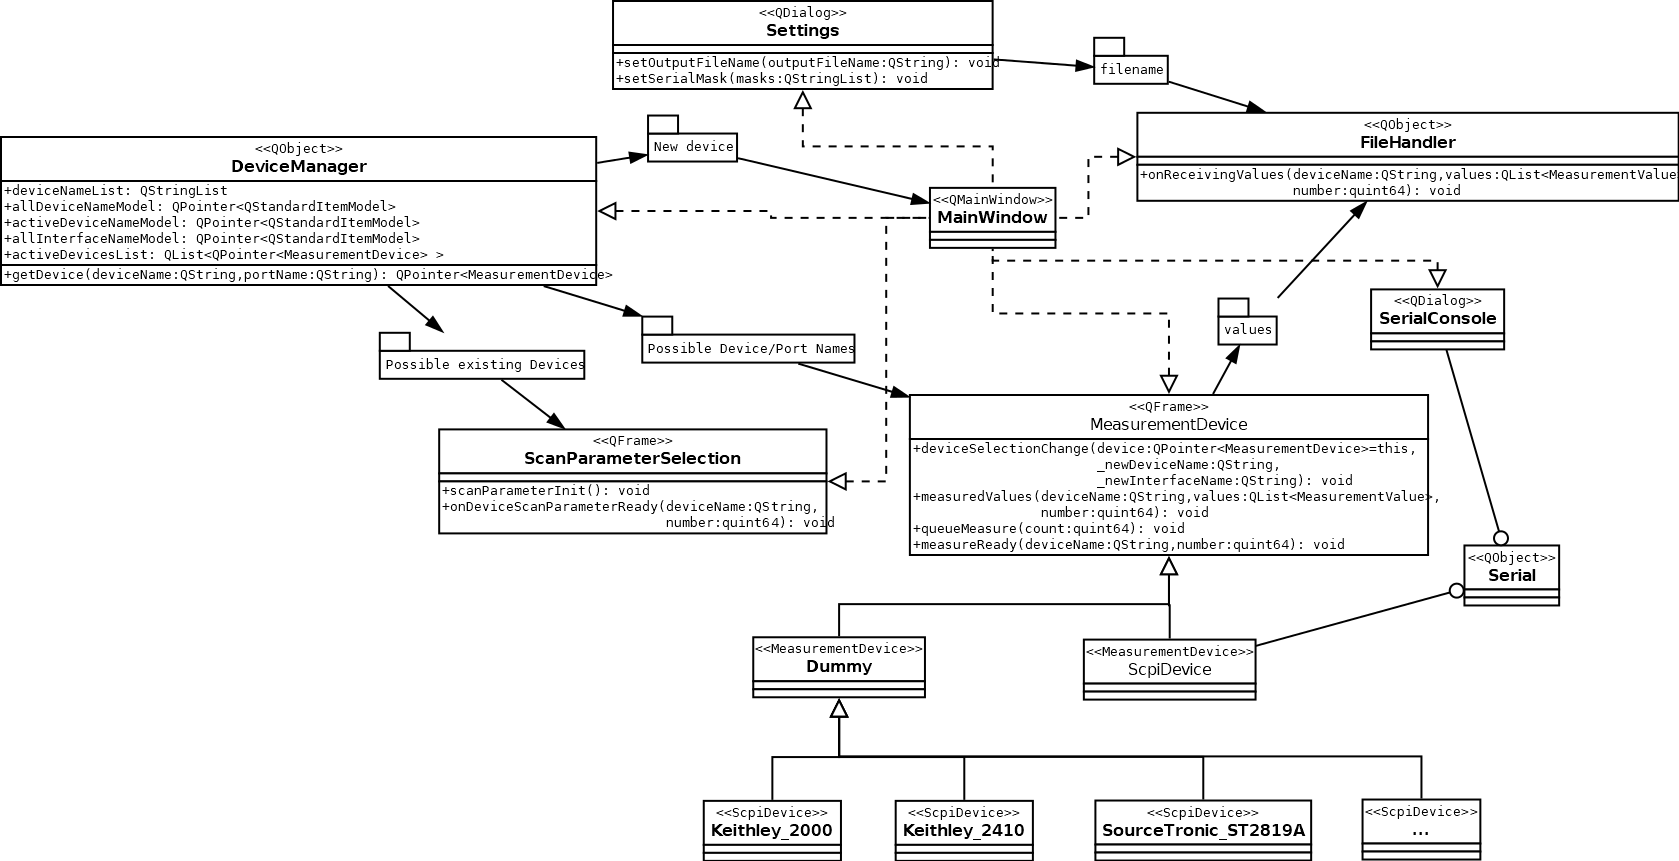
\includegraphics[width=\textwidth]{generalpurposecontrol.png}
	\caption{class diagram}
	\label{fig:classdiagram}
\end{figure}
\par\bigskip

The MainWindow class can contain objects of type MeasurementDevice and ScanParameterSelection in different areas of the GUI as can be seen in figure~\ref{fig:guicolored}.\par\bigskip

The MeasurementDevice is for itself a widget that has a graphical representation of the parameters one hardware device might have: a device name, port (address) and a table of values that can be written or read by the device, for example voltage or current. Also the information of read/write access possibility is in this table. MeasurementDevice has abstract functions for starting measurements and sending the results to some other class and is therefore the parent class of all device classes. Polymorphism is used to store all different child classes inside the same layout in the main window.\par\bigskip

The ScanParameterSelection class is used to set write-enabled parameters to certain values or ramping them during a measurement. A previously instantiated device can be selected from the drop down menu in ScanParameterSelection thanks to the DeviceManager class which holds an overview of all instantiated device objects and providing the item models for the drop down menus etc.\par\bigskip

When a measurement is started in the main window by clicking 'start measurement' all ScanParameterSelection widgets create basically a nested loop. At each measurement step only one ramping parameter will be changed, allowing ramping of multiple parameters on multiple devices controlled by only one application. The progress of the whole measurement procedure is tracked by a progress bar which is calculated at each increment, showing the overall progress.\newpage

\begin{figure}[h]
	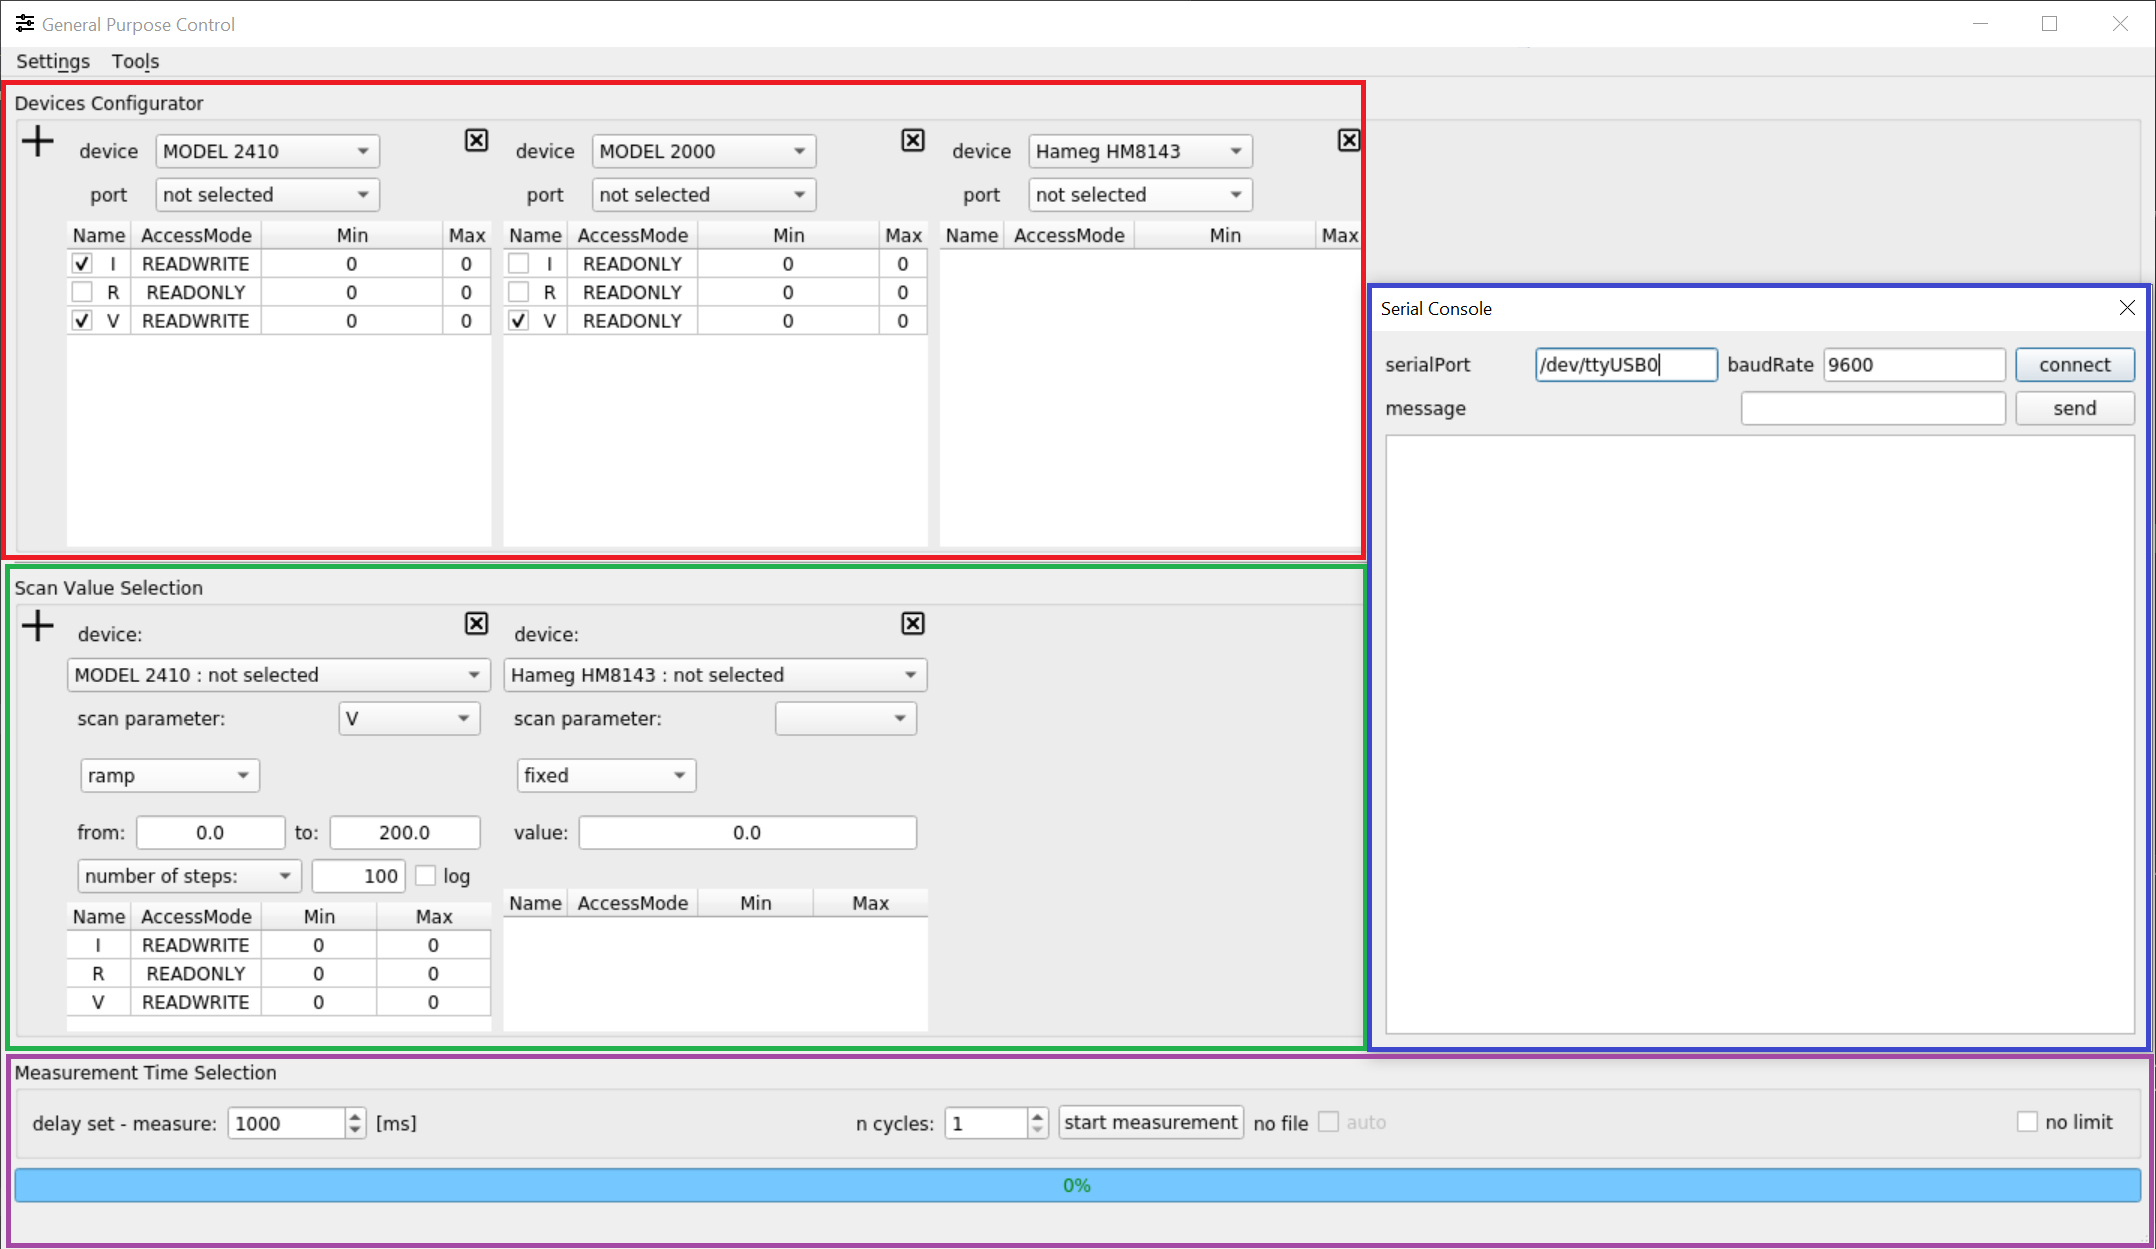
\includegraphics[width=\textwidth]{gui_all_colored.png}
	\caption{\\
		\color{Red}red\color{black}: Device selection area;\\
		\color{Green}green\color{black}: Scan parameter selection area;\\
		\color{Blue}blue\color{black}: Serial console pop-up dialog; \\
		\color{Purple}purple\color{black}: measurement / time selection and info area}
	\label{fig:guicolored}
\end{figure}
\par\bigskip

\newpage
\section{How to: Create new device class}
Since the program is designed to feature a variety of different interfaces, protocols and devices, inheritance is used to try to bundle multiple similar connected devices together. This prevents code from being redundant and creates a better structure of the code. The best example is the ScpiDevice class which is directly inherited from MeasurementDevice and features functions that all devices, which use the scpi protocol via uart, have.
\lstinputlisting[style=cppstyle]{content/code/scpidevice.h}
(functions for sending and receiving messages are the same for every scpi device but the content of the message changes)\par\bigskip
For devices that use different interfaces the process of adding a new device is somewhat similar but this section focuses on the ScpiDevice class because it is the standard protocol for lab devices.\par\bigskip
To add new devices to the program following steps must be done:
\begin{enumerate}
	\item Create a new class that inherits from some other device class like MeasurementDevice or ScpiDevice or other depending on the hardware interface and protocol used by the device. The device must have a device parameter map which defines the devices physical parameters like voltage or current etc. and how they can be accessed.
	\item Add the new device class to the DeviceManager to make it show up as possible device in the drop down menu.
	\item Define functions so that queueMeasure, and setScanParameter do the correct things and implement the other functions for communicating with the hardware device. For devices inherited from ScpiDevice only translate functions have to be implemented which create the message texts for different purposes.
\end{enumerate}
\par\bigskip
Which functions are required by the main window for measurements \\(that include readout and setting of scan parameter)?
How does one cycle work?
\begin{enumerate}
	\item Main window connects all relevant signals and slots and tells the \\
	ScanParameterSelection in the queue to initialize and set values.
	\item ScanParameterSelection tells the underlying devices to write a parameter value. When ready they will report the ready state to the main window.
	\item When all parameters are set a timer is started and after the timeout a measure command (signal) is sent to all MeasurementDevice objects.
	\item MeasurementDevice objects will queue the measure and report back to the main window when measure is completed. The measurement values will be sent to the FileHandler class for saving to file. Then start at 1 again (without initialization).
\end{enumerate}

\newpage
\subsection{Create new class}
\subsubsection{Create a new scpi protocol based class}
With the Keithley 2410 as an example for a scpi protocol based device it can be explained how to create a new class:
\lstinputlisting[style=cppstyle]{content/code/keithley_2410.h}\par\bigskip
Only the functions translateMeas, translateSet, translateInc, deviceName and the device parameter map are really relevant since all standard functionality for scpi protocol is handled in ScpiDevice class (e.g. communicating with the Serial interface, queueing messages etc.).\par\bigskip
The device parameter map defines the physical parameters a device can handle (interact with) such as for example voltage, current or resistance. It also shows if the parameter is read only or can be set by the device (high voltage supply for example). The other parameters in the device parameter map are the limits of the device which do not yet have any functionality but will prevent some bad things from happening in the future (for example open a warning if you try to apply higher voltage as output than another device can handle).
\par\bigskip
The translate functions are just there to define the device specific commands for measurement or scan parameter set functionality. For example ":MEAS:VOLT?" is the command string to initiate a voltage measurement on Keithley devices. The translateMeas function translates the abstract parameter name "V" for voltage to a measurement command string that this specific device understands. The same thing can be done for setting a voltage and this is done in function translateSet which also gets the to be set parameter value as an argument. The translateInc function has the sole purpose of translating a message received from the hardware device via uart into a numerical value. Often devices send the unit together with the value as a string so the value has to be parsed correctly then.
\newpage
\lstinputlisting[style=cppstyle]{content/code/keithley_2410.cpp}
\par\bigskip
There is also the function deviceName which must return the device designation returned by the hardware device when sending the universally (for scpi) valid "IDN?" command. It is used by ScpiDevice to validate the correct device connected to the selected port. Also important is setting up the init function and translate functions so that the correct terminator char is sent and received. This might take a bit of tweaking of the Serial class or ScpiDevice class to work for every hardware device.
\newpage
\subsubsection{Create a new class for any interface or protocol}
If the hardware device does not use uart or scpi inheriting from ScpiDevice is not an option. The class must be inherited directly from MeasurementDevice or somee other child of MeasurementDevice that is the generalized class for the specific interface or protocol. How to create a class directly inherited from MeasurementDevice will be shown at the example of the ScpiDevie class.
\par\bigskip
There are a few functions that must exist and have specific functionality because they are getting called by other classes. Also some signals have to be emitted at certain points.
\par\bigskip
\begin{itemize}
	\item setScanParameter function must send a command to the hardware device to set a certain parameter to a certain value.
	\lstinputlisting[style=cppstyle]{content/code/setscanparameter.cpp}
	scanParameterReady must be emitted when this is done or will be done soon. This will always contain the device designation and the event number.
	\par\bigskip
	\item queueMeasure function checks which parameters should be measured and remembers the active measurement parameters. It must somehow tell the hardware device to measure (synchronous or asynchronous). After measurement is complete the class \underline{must} emit a measureReady signal. How this is implemented is not important as long as queueMeasure function exists.
	\lstinputlisting[style=cppstyle]{content/code/queuemeasure.cpp}
	\par\bigskip
	\item onReceivedMessage is a function that will be probably be obsolete in future version of MeasurementDevice and is only relevant for asynchronous communication with the hardware interface.
	\par\bigskip
	\item connectBus is the abstract function for initialization of the serial interface. It is automatically called when the interface selection changes in the GUI. In this function the connection to the asynchronous serial interface can be opened. It must be made sure that the automatically emitted closeConnection signal closes the serial connection cleanly.
	\lstinputlisting[style=cppstyle]{content/code/connectbus.cpp}
	\par\bigskip
	\item checkDevice function is not needed but it is recommended to create some kind of function that checks if the connected device is correct and then signals this status to the widget.
	\lstinputlisting[style=cppstyle]{content/code/checkdevice.cpp}
\end{itemize}
\par\bigskip
To sum it up: it must be made sure that 
\begin{enumerate}
	\item setScanParameter sets the parameter (writes the parameter)
	\item queueMeasure function initiates a measurement
	\item scanParameterReady is emitted when scan parameter is written
	\item measureReady is emitted when all scheduled measurements for this iteration are finished
	\item all pure virtual functions in MeasurementDevice are created in the child class\\
	(or it will be an abstract class, you cannot instantiate an abstract class)
	\item the child class that represents a hardware device has a device parameter map as stated earlier
\end{enumerate}

\newpage
\subsection{Add class to DeviceManager getDevice function}
Make sure that the getDevice function in the DeviceManager class returns the correct newly created class (which must be directly or indirectly inherited from MeasurementDevice to be stored in a pointer of type MeasurementDevice, see polymorphism). This will make the device show up in the drop down menu when adding a new device to the layout in the main window (by clicking the upper plus sign button).
\par\smallskip
\lstinputlisting[style=cppstyle]{content/code/devicemanager.cpp}
\appendix
\section{Sources}
%\lstinputlisting[style=cppstyle]{content/code/main.cpp}
\begin{cpp}
	#include "mainwindow.h"
	#include <QApplication>
	
	int main(int argc, char *argv[])
	{
		QApplication a(argc, argv);
		MainWindow w;
		w.show();
		
		return a.exec();
	}
\end{cpp}
\end{document}
%% Dokument ENDE %%%%%%%%%%%%%%%%%%%%%%%%%%%%%%%%%%%%%%%%%%%%%%%%%%%%%%%%%%

